\documentclass[12pt]{article}
 
\usepackage[table]{xcolor}
\usepackage[margin=1in]{geometry} 
\usepackage{amsmath,amsthm,amssymb,wasysym}
\usepackage{pgf,tikz,pgfplots}
\usepackage{mathrsfs}
\usepackage{mathtools}
\usepackage{listings}
\usepackage{colortbl}
\usepackage{verbatim}
\usetikzlibrary{arrows, angles, quotes, decorations.pathreplacing, math, patterns}
\usepackage{framed}
\usepackage{graphicx}
\usepackage{multirow}
\graphicspath{ {./images/} }

\lstset{basicstyle=\footnotesize}
\usetikzlibrary{calc}

\newcommand{\N}{\mathbb{N}}
\newcommand{\Z}{\mathbb{Z}}
\newcommand{\I}{\mathbb{I}}
\newcommand{\R}{\mathbb{R}}
\newcommand{\Q}{\mathbb{Q}}
\newcommand{\p}{^{\prime}}
\DeclarePairedDelimiter{\ceil}{\lceil}{\rceil}

 
\begin{document}
 
\title{Induction\\
    \large MATH CS101A Problem Solving I}
\author{Harry Coleman}
\date{November 19, 2019}

\maketitle

\section*{Problem 2}
\fbox{
    \parbox{\textwidth} {
        Let 13 points $P_1, P_2, \dots, P_{13}$ be given in the plane, and suppose they are connected by the segments $P_1P_2, P_2P_3, \dots, P_{12}P_{13}, P_{13}P_1$. Is it possible to draw a straight line which passes through the interior of each of these segments?
    }
}
\\

If we assume that it is possible to draw such a line, call it $A$, through each segment, then the endpoints of each segment must lie on opposite sides of $A$. So we must have
\begin{center}
    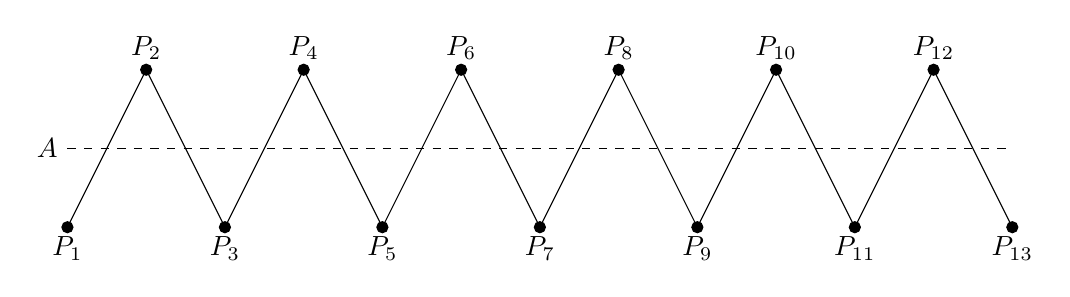
\begin{tikzpicture}
        \coordinate (P1) at (0,0);
        \coordinate (P2) at (1,2);
        \coordinate (P3) at (2,0);
        \coordinate (P4) at (3,2);
        \coordinate (P5) at (4,0);
        \coordinate (P6) at (5,2);
        \coordinate (P7) at (6,0);
        \coordinate (P8) at (7,2);
        \coordinate (P9) at (8,0);
        \coordinate (P10) at (9,2);
        \coordinate (P11) at (10,0);
        \coordinate (P12) at (11,2);
        \coordinate (P13) at (12,0);
        
        \draw[fill=black] (P1) circle (2pt) node[anchor=north]{$P_1$};
        \draw[fill=black] (P2) circle (2pt) node[anchor=south]{$P_2$};
        \draw[fill=black] (P3) circle (2pt) node[anchor=north]{$P_3$};
        \draw[fill=black] (P4) circle (2pt) node[anchor=south]{$P_4$};
        \draw[fill=black] (P5) circle (2pt) node[anchor=north]{$P_5$};
        \draw[fill=black] (P6) circle (2pt) node[anchor=south]{$P_6$};
        \draw[fill=black] (P7) circle (2pt) node[anchor=north]{$P_7$};
        \draw[fill=black] (P8) circle (2pt) node[anchor=south]{$P_8$};
        \draw[fill=black] (P9) circle (2pt) node[anchor=north]{$P_9$};
        \draw[fill=black] (P10) circle (2pt) node[anchor=south]{$P_{10}$};
        \draw[fill=black] (P11) circle (2pt) node[anchor=north]{$P_{11}$};
        \draw[fill=black] (P12) circle (2pt) node[anchor=south]{$P_{12}$};
        \draw[fill=black] (P13) circle (2pt) node[anchor=north]{$P_{13}$};
        
        \draw[] (P1)--(P2)--(P3)--(P4)--(P5)--(P6)--(P7)--(P8)--(P9)--(P10)--(P11)--(P12)--(P13);
        
        
        \draw[dashed] (0,1) node[anchor=east]{$A$} -- (12,1);
    \end{tikzpicture}
\end{center}

We can see that starting from $P_1$, every odd-numbered vertex is on the same side of $A$, and every even-numbered vertex is on the opposite side. So since $P_1$ and $P_{13}$ are necessarily on the same side of $A$, the segment connecting them cannot cross $A$. This contradicts our assumption that $A$ could cross all the segments. Therefore, it is not possible to draw such a straight line through each segment. In fact, it would be impossible for any such odd-number collection of segments.

\newpage
\section*{Problem 3}
\fbox{
    \parbox{\textwidth} {
        Let there be given nine lattice points in the three-dimensional Euclidean space. Show that there is a lattice point on the interior of one of the line segments joining two of these points.
    }
}
\\

Consider two arbitrary lattice points
\begin{align*}
    P_1 &= (x_1, y_1, z_1) \\
    P_2 &= (x_2, y_2, z_2)
\end{align*}

We can define the line passing through these two points by
\[(x,y,z) = (x_1, y_1, z_1) + t(x_2-x_1, y_2-y_1, z_2-z_1)\]
and with $0<t<1$, we get points on the interior of the line segment joining $P_1$ and $P_2$. If we let $t=\frac{1}{2}$, then we get such a point,
\[M = \left(x_1 + \frac{x_2-x_1}{2}, \quad y_1 + \frac{y_2-y_1}{2}, \quad z_1 + \frac{z_2-z_1}{2}\right)\]
$M$ is a lattice point if and only if $(x_2-x_1)$, $(y_2-y_1)$, and $(z_2-z_1)$ are all even, which is to say
\[(x_1, y_1, z_1) \equiv (x_2, y_2, z_2) \pmod{2}\]

So for two points, $P_1$ and $P_2$, there is a lattice point on the interior of the segment segment joining $P_1$ to $P_2$ if 
\[(x_1, y_1, z_1) \equiv (x_2, y_2, z_2) \pmod{2}\]

Since there are eight possible values for an integral ordered triple of modulo 2 and we have nine lattice points which can be represented as integral ordered triples in mod 2, then by the pigeonhole principle, we must have at least two points which are equivalent modulo 2, and have a lattice point between them. So there is at least one lattice point on the interior of the line segment joining two points in the set of nine lattice points.

\newpage
\section*{Problem 4}
\fbox{
    \parbox{\textwidth} {
        Place a knight on each square of a 7-by-7 chessboard. Is it possible for each knight to simultaneously make a legal move?
    }
}
\\

Consider a 7-by-7 chessboard.
\begin{center}
    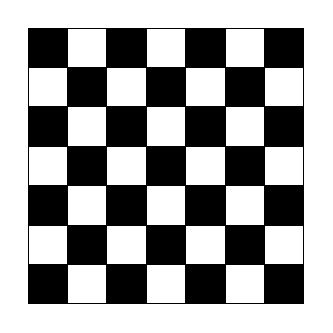
\begin{tikzpicture}
        \draw[fill=black] (0,0) rectangle (3.5,3.5);
        
        \foreach \x in {0, 1, 2, 3}{
            \foreach \y in {0.5, 1.5, 2.5}{
                \draw[fill=white, line width=0] (\x,\y) rectangle (\x+0.5, \y+0.5);
                \draw[fill=white, line width=0] (\y,\x) rectangle (\y+0.5, \x+0.5);
            }
        }
    \end{tikzpicture}
\end{center}

A knight on a white square can only move to a knight on a black square, and vice versa. On a 7x7 chessboard, there are 25 black squares but only 24 white square. So when all of the knights from the black squares move to white squares, by the pigeonhole principle, at least one white square will have two knights from black squares. This would not be a legal move, so it is not possible for all the knights to simultaneously make legal moves.

\section*{Problem 5}
\fbox{
    \parbox{\textwidth} {
        Place a knight on a 7-by-7 chessboard. Is it possible, in 49 consecutive knight moves, to visit each square of the board and return to the original square?
    }
}
\\

We'll call the sequence of unique squares the knight travels through $(a_1, a_2, a_3, \dots, a_{49})$. Each $a_i$ is unique and the knight moves from $a_i$ to $a_{i+1}$, as well as from $a_{49}$ to $a_1$ as the final move. Since, for every move, the color of the square the knight is on switches, then for all odd $i$, $a_i$ are the same color as $a_1$, the opposite color for even $i$. This means that $a_{49}$ and $a_1$ are the same color, so the knight cannot move from $a_{49}$ to $a_1$. So it is not possible to return to the original square after such a series of moves.

\newpage
\section*{Problem 6}
\fbox{
    \parbox{\textwidth} {
        Place a knight on a 4-by-$n$ chessboard. Is it possible, in $4n$ consecutive knight moves, to visit each square of the board and return to the original square?
    }
}
\\

Assuming it is possible to move a knight in such a way, we'll represent the path of the knight as the sequence of unique squares $(a_1, a_2, a_3,\dots, a_{4n})$ where each $a_i$ is a square on the board. The knight moves from each $a_i$ to $a_{i+1}$ and from $a_{4n}$ to $a_1$.
\[a_1 \longrightarrow a_2 \longrightarrow a_3 \longrightarrow \cdots \longrightarrow a_{4n} \longrightarrow a_1\]

Consider the following denotation of a 4-by-$n$ chessboard.
\begin{center}
    \begin{tabular}{c|c|c|c|c|}
        \multicolumn{5}{c}{\hspace{1.65em}4} \\
        \cline{2-5}
        \multirow{7}{*}{$n$} &
        $\CIRCLE$ & $\Circle$ & $\times$ & $\times$ \\
        \cline{2-5}
        & $\times$ & $\times$ & $\Circle$ & $\CIRCLE$ \\
        \cline{2-5}
        & $\CIRCLE$ & $\Circle$ & $\times$ & $\times$ \\
        \cline{2-5}
        & $\times$ & $\times$ & $\Circle$ & $\CIRCLE$ \\
        \cline{2-5}
        & $\CIRCLE$ & $\Circle$ & $\times$ & $\times$ \\
        \cline{2-5}
        & $\times$ & $\times$ & $\Circle$ & $\CIRCLE$ \\
        \cline{2-5}
        \multicolumn{5}{c}{\hspace{1.65em}$\vdots$}
    \end{tabular}
\end{center}

We can see that a knight on a $\CIRCLE$ square must have come from a $\Circle$ square and can only move to a different $\Circle$ square. So for each $\CIRCLE$ square, we must have
\[\cdots \Circle \longrightarrow \CIRCLE \longrightarrow \Circle \cdots\]

Since each $a_i$ has unique $a_x$ and $a_y$ such that $a_x \longrightarrow a_i \longrightarrow a_y$ and there are an equal number of $\CIRCLE$ and $\Circle$ squares, then, by the pigeonhole principle, for each $\Circle$ square, we must have
\[\cdots \CIRCLE \longrightarrow \Circle \longrightarrow \CIRCLE \cdots\]

This means that a knight on a $\CIRCLE$ or $\Circle$ square can only move to other $\CIRCLE$ and $\Circle$ squares, and will never reach any of the $\times$ squares. So it is not possible to have the knight visit each square exactly once and return to the original square.


\section*{Problem 7}
\fbox{
    \parbox{\textwidth} {
        Let $n$ be an odd integer greater than 1, and let $A$ be an $n$-by-$n$ symmetric matrix such that each row and each column of $A$ consists of some permutation of the integers $1,2,\dots,n$. Show that each one of the integers $1,\dots,n$ must appear in the main diagonal of $A$.
    }
}
\\

Each integer $1,2,3,\dots,n$ occurs $n$(odd) times in the matrix. If a number occurs in a location not on the main diagonal, then there must be a corresponding occurrence of the number which is on the other side of the main diagonal. So each number has an even number of occurrences not on the main diagonal. But since each number occurs an odd number of times overall, there must be an odd number of occurrences of each number on the main diagonal. Since there are $n$ locations on the main diagonal, and $n$ numbers with at least one occurrence on the main diagonal, then by the pigeonhole principle, each number occurs exactly once on the main diagonal.


\newpage
\section*{Problem 8}
\fbox{
    \parbox{\textwidth} {
        Let $a_1, a_2, a_3, \dots, a_{2n+1}$ be a set of integers with the following property (P): if any of them is removed, the remaining ones can be divided into two sets of $n$ integers with equal sums. Prove that $a_1=a_2=\dots=a_{2n+1}$.
    }
}
\\

We'll define the collection of integers to be
\[A=\{a_1, a_2, a_3, \dots, a_{2n+1}\}\]
and the overall sum of this set to be
\[m = \sum A\]
We are given that P(A) is true, which means that for each $a_i \in A$, we can find a partition of $A\setminus\{a_i\}$ into $A_x$ and $A_y$ such that
\begin{equation} \label{size}
    |A_x| = |A_y| = n
\end{equation}
\begin{equation} \label{sum}
    \sum A_x = \sum A_y = \frac{m - a_i}{2}
\end{equation}

Firstly, we will prove that some linear function applied to $A$, say $A\p=bA+c$, we would still have $P(A\p)$ true. We'll define
\[A\p = \{(ba_i +c) : a_i\in A\} \quad \text{where $b,c\in\R$}\]
\[m\p = \sum A\p = bm + c(2n+1)\]
For each $a_i\p \in A\p$, we can find partitions of $A\p\setminus\{a_i\p\}$ based on the partitions for $A\setminus\{a_i\}$. Say
\[A_x\p = \{a_i\p\in A\p: a_i\in A_x\}\]
\[A_y\p = \{a_i\p\in A\p: a_i\in A_y\}\]
so
\begin{align*}
    |A_x\p| &= |A_x| \\
    & = |A_y| \\
    & = |A_y\p| = n
\end{align*}
which satisfies \eqref{size} for $P$. And we can also find

\begin{align*}
    \sum A_x\p &= b\left(\sum A_x\right) + cn \\
    & = b\left(\sum A_y\right) + cn \\
    & = \sum A_y\p \\
    & = b\left(\frac{m - a_i}{2}\right) + cn \\
    & = \frac{bm - ba_i + 2cn}{2} \\
    & = \frac{bm - (ba_i+c) + 2cn + c}{2} \\
    & = \frac{bm + c(2n+1) - a_i\p}{2} \\
    & = \frac{m\p - a_i\p}{2} \\
\end{align*}
which satisfies \eqref{sum} for $P$. So $P(A\p)$ is true.

Secondly, we want to show that for any set of integers which satisfies $P$, all the elements have the same parity. Looking at \eqref{sum}, we must have that the sum of all of the elements in the set, minus any one element, is divisible by 2, and therefore even. So if the sum of all the elements in even, then all the elements must be even. If the sum of all the elements is odd, then all the elements must be odd. This is true because if we had an element which had a different parity to the sum, then the sum minus that element would be odd, and not divisible by 2. Therefore, all the elements in a set of integers which satisfies $P$ have the same parity.

With these two properties, we will look at our original set of integers, and assume that they are not all the same value.
\[A = \{a_1, a_2, a_3, \dots, a_{2n+1}\}\]

Since we can apply a linear operation, and have the property continue to hold, we'll say
\begin{align*}
    A\p = A-a_1 &= \{a_1\p, a_2\p, a_3\p, \dots, a_{2n+1}\p\} \\
                &= \{0, a_2-a_1, a_3-a_1, \dots, a_{2n+1}-a_1\}
\end{align*}

Since we have $a_1\p=0$, which is even, then all other values in $A\p$ are also even. And since not all the elements are equal, there are some which are not equal to zero. These elements are of the fom $a_i\p=2^{k_i}b_i$ for some $k_i\in\Z^+$ and odd $b_i\in(\Z\setminus\{0\})$. Looking at the element of such form with the smallest $k_i$ value, $a_l\p$, we can divide all the elements in $A\p$ by $2^{k_l}$ to get 
\[A\p\p = A\p \cdot \frac{1}{2^{k_l}}\]
where $a_l\p\p=1$, and $a_1\p\p=0$. However since $P(A\p\p)$, then all the elements must have the same parity, but $a_l\p\p$ and $a_1\p\p$ have different parity, which is a contradiction.

So our assumption that not all the values in $A$ are equal is false. Therefore, all the values in $A$ are equal.



\end{document}